% ===========================================================================
% Part VI - Sequence Modeling: Recurrent Neural Networks (Experiment 14)
% ===========================================================================

\part{Sequence Modeling: Recurrent Neural Networks}

% ---------------------------------------------------------------------------
\chapter{Recurrent Neural Network (RNN)}\label{exp:14}

\runninghead{Experiment 14: Recurrent Neural Network (RNN)}

\quickfacts
  {Dataset}{Synthetic 20-step sequences (1,200; label = positive sum) and Monthly Airline Passengers (12-month windows)}
  {Key parameters}{Vanilla RNN vs LSTM; 2 layers, hidden 64 (forecasting) / 32 (classification); Adam; MSE / BCE loss}
  {Headline result}{Forecasting: LSTM RMSE 44.12 vs RNN 69.93 passengers; Classification: LSTM 0.9450 vs RNN 0.9300}

\section{Objective}
Build recurrent networks for sequential data --- sequence classification and time-series
forecasting --- and compare a vanilla RNN with an LSTM.

\section{Suggested Dataset}
(a) Synthetic sequence benchmark: 1,200 sequences of length 20, label = 1 if the sum is
positive (1,000 train / 200 test). (b) Monthly Airline Passengers
(\texttt{data/airline\_passengers.csv}): 144 months, 12-month sliding windows, chronological
80/20 split.

\section{Required Libraries}
PyTorch, numpy, pandas, matplotlib (the manual's TensorFlow/Keras example is implemented
equivalently in PyTorch, the framework installed in this environment).

\section{Brief Theory}
A recurrent network processes a sequence one step at a time while maintaining a hidden state,
\[
h_t = \tanh\bigl(W_{ih} x_t + b_{ih} + W_{hh} h_{t-1} + b_{hh}\bigr), \qquad
\hat{y} = W_{ho} h_T + b_o .
\]
Training uses backpropagation through time (BPTT). Repeated multiplication by $W_{hh}$ makes
gradients vanish (or explode) over long sequences. The \textbf{LSTM} solves this with gates ---
forget $f_t$, input $i_t$ and output $o_t$ --- and an additive cell state
$c_t = f_t \odot c_{t-1} + i_t \odot \tilde{c}_t$, which lets gradients flow across many steps.

\section{Procedure}
\begin{enumerate}
  \item Generate 1,200 labeled 20-step sequences (label = 1 if the sum is positive) and split
        1,000/200.
  \item Build vanilla RNN and LSTM classifiers (hidden 32, linear sigmoid output); train
        10 epochs with Adam and binary cross-entropy; report test accuracy.
  \item For forecasting, normalize the passenger series and build 12-month sliding windows with
        a chronological 80/20 split.
  \item Train RNN and LSTM forecasters (2 layers, hidden 64, MSE, Adam, 120 epochs).
  \item Report RMSE/MAE and plot the forecast trajectories.
\end{enumerate}

\section{Reference Implementation}
\begin{codebox}[title={Recurrent model definitions (classification and forecasting)}]
self.rnn = nn.RNN(1, hidden, batch_first=True) if cell == 'rnn' else nn.LSTM(1, hidden, batch_first=True)
self.fc = nn.Linear(hidden, 1)          # classification output

self.lstm = nn.LSTM(input_size=1, hidden_size=64, num_layers=2, batch_first=True)
self.fc = nn.Linear(64, 1)              # forecasting output
\end{codebox}

\section{Evaluation / Expected Output}
\begin{table}[htbp]
  \centering
  \caption{Sequence classification on the synthetic benchmark (200 test sequences).}
  \begin{tabular}{|l|r|}
    \hline
\rowcolor{mlblue!8}    \textbf{Model} & \textbf{Test accuracy} \\
    \hline
    Vanilla RNN & 0.9300 \\
\hline
    LSTM & \best{0.9450} \\
    \hline
  \end{tabular}
\end{table}

\begin{table}[htbp]
  \centering
  \caption{Airline passenger forecasting on the chronological test horizon (27 windows).}
  \begin{tabular}{|l|r|r|}
    \hline
\rowcolor{mlblue!8}    \textbf{Model} & \textbf{RMSE (passengers)} & \textbf{MAE} \\
    \hline
    Vanilla RNN & 69.93 & 62.36 \\
\hline
    LSTM & \best{44.12} & \best{36.78} \\
    \hline
  \end{tabular}
\end{table}

\begin{figure}[htbp]
  \centering
  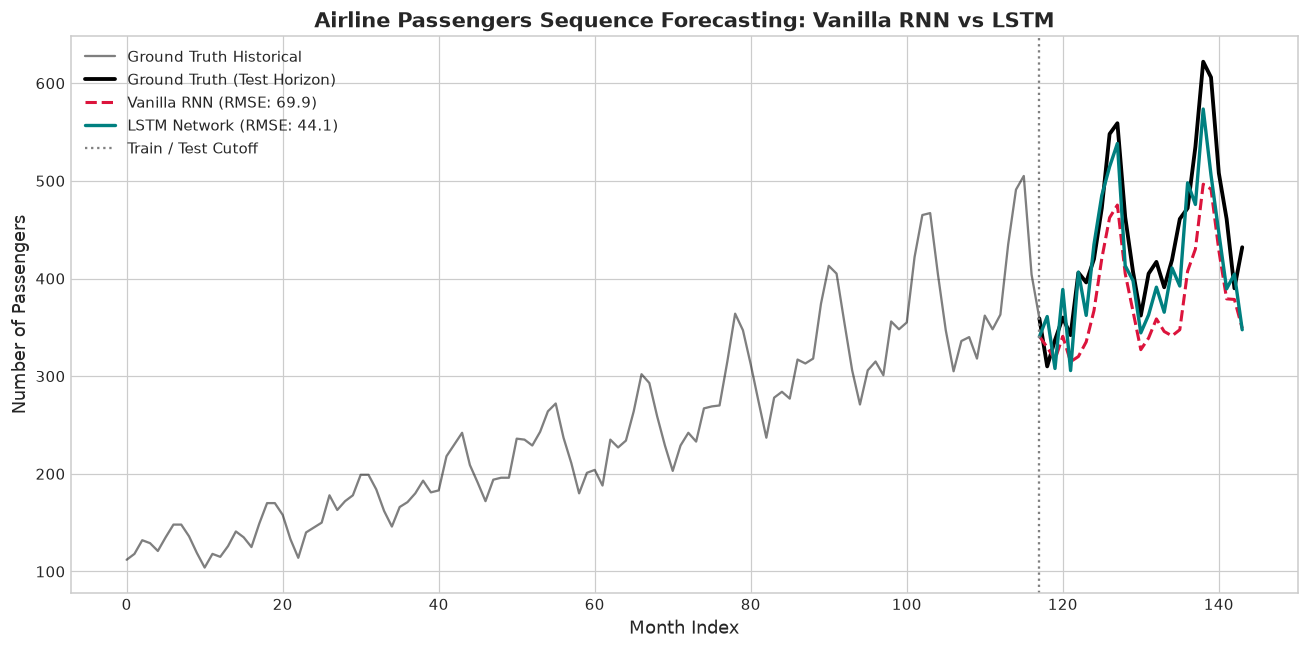
\includegraphics[width=0.95\textwidth]{figures/exp14_forecast.png}
  \caption{Airline passenger forecasting: ground truth versus the RNN and LSTM forecasts on
  the test horizon.}
  \label{fig:exp14-forecast}
\end{figure}

The LSTM outperforms the vanilla RNN on both tasks: $+1.5$ accuracy points on classification
and about $37\%$ lower RMSE on forecasting. The gap is larger on forecasting because that task
needs 12-step seasonal memory, exactly where gating prevents vanishing gradients. On the easy
synthetic benchmark both models do well because the decision rule (sum $> 0$) is nearly linear.

\section{Viva / Discussion Questions}
\begin{description}
  \item[Why does an RNN have memory?] Its hidden state is carried across time steps, so each
  output depends on previous inputs, not only the current one.
  \item[What is a hidden state?] The internal vector summarizing the sequence seen so far; it
  is updated at every step and used to produce outputs.
  \item[Why are LSTM/GRU often preferred for long dependencies?] Their gates control what is
  stored or forgotten and the additive cell state lets gradients flow across many steps,
  avoiding the exponential decay of vanilla RNN gradients.
  \item[Why is the train/test split chronological?] Shuffling sequences would leak future
  values into training and produce an optimistic, invalid evaluation.
\end{description}

\FloatBarrier
\section{Complete Code Listing}
% ===========================================================================
% exp14_rnn.tex - complete code listings for Experiment 14
% Source: notebooks/06_recurrent_neural_network.ipynb (executed)
% ===========================================================================

\begin{codebox}[title={Core numerical and plotting libraries}]
# ---- Core numerical and plotting libraries ----
import numpy as np
import pandas as pd
import matplotlib.pyplot as plt
import seaborn as sns

# ---- Scaling + regression metrics ----
from sklearn.preprocessing import MinMaxScaler
from sklearn.metrics import root_mean_squared_error, mean_absolute_error, accuracy_score

# ---- PyTorch for the recurrent models ----
import torch
import torch.nn as nn
import torch.optim as optim
from torch.utils.data import DataLoader, TensorDataset

# Aesthetics setup (consistent look across all notebooks)
plt.style.use('seaborn-v0_8-whitegrid' if 'seaborn-v0_8-whitegrid' in plt.style.available else 'default')
plt.rcParams['font.sans-serif'] = 'DejaVu Sans'
plt.rcParams['figure.figsize'] = (10, 5)
plt.rcParams['figure.dpi'] = 110

# Reproducibility
torch.manual_seed(42)
torch.cuda.manual_seed_all(42)  # reproducible GPU training
np.random.seed(42)
device = torch.device('cuda' if torch.cuda.is_available() else 'cpu')
print(f"PyTorch version: {torch.__version__} on {device}")

# ---- Load the monthly airline passengers time series ----
df_air = pd.read_csv('../data/airline_passengers.csv')
print("Dataset Head:")
display(df_air.head())

# Extract the target series as float32 (shape: N x 1)
passengers = df_air['Passengers'].values.astype(np.float32).reshape(-1, 1)
# ---- Normalize to [0, 1] (RNNs train much better on small inputs) ----
scaler = MinMaxScaler(feature_range=(0, 1))
scaled_data = scaler.fit_transform(passengers)

# ---- Function to build supervised sliding-window sequences ----
# For each time step t: X = values [t-seq_len ... t-1], y = value at t
def create_sequences(data, seq_length=12):
    xs, ys = [], []
    for i in range(len(data) - seq_length):
        x = data[i:(i + seq_length)]
        y = data[i + seq_length]
        xs.append(x)
        ys.append(y)
    return np.array(xs), np.array(ys)

SEQ_LENGTH = 12  # 12-month lookback = one full annual seasonal cycle
X_seq, y_seq = create_sequences(scaled_data, seq_length=SEQ_LENGTH)

# ---- Temporal split: 80% train, 20% test WITHOUT shuffling (time order matters) ----
train_size = int(len(X_seq) * 0.80)
X_train, X_test = X_seq[:train_size], X_seq[train_size:]
y_train, y_test = y_seq[:train_size], y_seq[train_size:]

print(f"Total sequences created: {len(X_seq)}")
print(f"Training sequences:      {X_train.shape[0]} (Shape: {X_train.shape})")
print(f"Testing sequences:       {X_test.shape[0]}  (Shape: {X_test.shape})")

# ---- DataLoader for mini-batch training (shuffle only the training set) ----
train_loader = DataLoader(
    TensorDataset(torch.tensor(X_train, dtype=torch.float32), torch.tensor(y_train, dtype=torch.float32)),
    batch_size=16,
    shuffle=True
)
\end{codebox}

\begin{codebox}[title={Vanilla RNN and LSTM model definitions}]
class VanillaRNN(nn.Module):
    """Elman RNN: 2 stacked recurrent layers + a linear output layer."""
    def __init__(self, input_size=1, hidden_size=64, num_layers=2):
        super(VanillaRNN, self).__init__()
        self.rnn = nn.RNN(input_size, hidden_size, num_layers, batch_first=True)
        self.fc = nn.Linear(hidden_size, 1)   # map final hidden state to a scalar forecast

    def forward(self, x):
        out, _ = self.rnn(x)                 # out: (batch, seq_len, hidden)
        out = self.fc(out[:, -1, :])         # use ONLY the last time step's hidden state
        return out

class LSTMModel(nn.Module):
    """LSTM: same interface, but gated cells preserve long-term information."""
    def __init__(self, input_size=1, hidden_size=64, num_layers=2):
        super(LSTMModel, self).__init__()
        self.lstm = nn.LSTM(input_size, hidden_size, num_layers, batch_first=True)
        self.fc = nn.Linear(hidden_size, 1)

    def forward(self, x):
        out, _ = self.lstm(x)
        out = self.fc(out[:, -1, :])
        return out

# Instantiate both models on the selected device so they can be compared fairly
rnn_model = VanillaRNN().to(device)
lstm_model = LSTMModel().to(device)
print("Models instantiated successfully!")
\end{codebox}

\begin{codebox}[title={Generic training function shared by both architectures}]
# ---- Generic training function shared by both architectures ----
def train_model(model, loader, epochs=120, lr=0.005):
    criterion = nn.MSELoss()                          # regression -> mean squared error
    optimizer = optim.Adam(model.parameters(), lr=lr) # Adam optimizer
    losses = []

    for epoch in range(epochs):
        model.train()
        total_loss = 0.0
        for x_b, y_b in loader:
            x_b, y_b = x_b.to(device), y_b.to(device)

            optimizer.zero_grad()          # clear previous gradients
            pred = model(x_b)              # forward pass through the recurrent net
            loss = criterion(pred, y_b)    # MSE between forecast and truth
            loss.backward()                # backpropagation through time (BPTT)
            optimizer.step()               # update weights

            total_loss += loss.item() * len(x_b)   # de-average the batch loss

        epoch_loss = total_loss / len(loader.dataset)
        losses.append(epoch_loss)          # track loss per epoch for plotting

    return losses

# ---- Train both architectures with identical hyperparameters ----
print("Training Vanilla RNN...")
rnn_losses = train_model(rnn_model, train_loader, epochs=120, lr=0.005)

print("Training LSTM Model...")
lstm_losses = train_model(lstm_model, train_loader, epochs=120, lr=0.005)
print("Training completed!")
\end{codebox}

\begin{codebox}[title={Evaluate both models on the test horizon}]
# ---- Evaluate both models on the test horizon ----
rnn_model.eval()
lstm_model.eval()

with torch.no_grad():   # inference only - no gradients
    x_test_t = torch.tensor(X_test, dtype=torch.float32).to(device)
    pred_rnn_scaled = rnn_model(x_test_t).cpu().numpy()    # normalized predictions
    pred_lstm_scaled = lstm_model(x_test_t).cpu().numpy()

# ---- Invert scaling to get real passenger counts ----
y_test_true = scaler.inverse_transform(y_test)
pred_rnn = scaler.inverse_transform(pred_rnn_scaled)
pred_lstm = scaler.inverse_transform(pred_lstm_scaled)

# ---- Compute error metrics in the original unit (passengers) ----
rmse_rnn = root_mean_squared_error(y_test_true, pred_rnn)
mae_rnn  = mean_absolute_error(y_test_true, pred_rnn)

rmse_lstm = root_mean_squared_error(y_test_true, pred_lstm)
mae_lstm  = mean_absolute_error(y_test_true, pred_lstm)

# ---- Summary table (lower errors are better) ----
eval_df = pd.DataFrame([
    {"Model": "Vanilla RNN", "RMSE (Passengers)": rmse_rnn, "MAE (Passengers)": mae_rnn},
    {"Model": "LSTM Network", "RMSE (Passengers)": rmse_lstm, "MAE (Passengers)": mae_lstm}
]).set_index("Model")

print("Time Series Forecasting Performance Comparison:")
display(eval_df.style.highlight_min(subset=['RMSE (Passengers)', 'MAE (Passengers)'], color='lightgreen'))

# ---- Plot ground truth vs. both forecast trajectories ----
# Map each test target back to its true position on the month axis:
# sequence i predicts month (i + SEQ_LENGTH)
test_indices = range(train_size + SEQ_LENGTH, len(passengers))

plt.figure(figsize=(12, 6))
# Full historical series in the background
plt.plot(range(len(passengers)), passengers, label='Ground Truth Historical', color='black', alpha=0.5, lw=1.5)

# Test-period ground truth
plt.plot(test_indices, y_test_true, label='Ground Truth (Test Horizon)', color='black', lw=2.5)

# Model forecasts
plt.plot(test_indices, pred_rnn, label=f'Vanilla RNN (RMSE: {rmse_rnn:.1f})', color='crimson', lw=2, linestyle='--')
plt.plot(test_indices, pred_lstm, label=f'LSTM Network (RMSE: {rmse_lstm:.1f})', color='teal', lw=2.2)

# Vertical line marking where the train period ends and test begins
plt.axvline(x=train_size + SEQ_LENGTH, color='gray', linestyle=':', label='Train / Test Cutoff')
plt.title("Airline Passengers Sequence Forecasting: Vanilla RNN vs LSTM", fontsize=14, fontweight='bold')
plt.xlabel("Month Index", fontsize=12)
plt.ylabel("Number of Passengers", fontsize=12)
plt.legend()
plt.tight_layout()
plt.show()
\end{codebox}

\begin{codebox}[title={Sequence classification benchmark (manual experiment)}]
# ---- Sequence classification benchmark (manual experiment) ----
rng = np.random.default_rng(42)
X_cls = rng.normal(size=(1200, 20, 1)).astype("float32")
y_cls = (X_cls.sum(axis=1).ravel() > 0).astype("float32")

X_tr_c, X_te_c = X_cls[:1000], X_cls[1000:]
y_tr_c, y_te_c = y_cls[:1000], y_cls[1000:]
print(f"Sequence classification data: train {X_tr_c.shape}, test {X_te_c.shape}")

class RNNClassifier(nn.Module):
    """Vanilla RNN or LSTM classifier over a 20-step sequence."""
    def __init__(self, cell='rnn', hidden=32):
        super().__init__()
        self.rnn = nn.RNN(1, hidden, batch_first=True) if cell == 'rnn' else nn.LSTM(1, hidden, batch_first=True)
        self.fc = nn.Linear(hidden, 1)

    def forward(self, x):
        out, _ = self.rnn(x)
        return self.fc(out[:, -1, :]).squeeze(-1)

def train_classifier(model, epochs=10):
    """Train a sequence classifier and return test accuracy."""
    model = model.to(device)
    optimizer = optim.Adam(model.parameters(), lr=0.005)
    loss_fn = nn.BCEWithLogitsLoss()
    loader = DataLoader(TensorDataset(torch.tensor(X_tr_c), torch.tensor(y_tr_c)), batch_size=32, shuffle=True)
    for epoch in range(epochs):
        model.train()
        for xb, yb in loader:
            xb, yb = xb.to(device), yb.to(device)
            optimizer.zero_grad()
            loss = loss_fn(model(xb), yb)
            loss.backward()
            optimizer.step()
    model.eval()
    with torch.no_grad():
        logits = model(torch.tensor(X_te_c).to(device))
        preds = (torch.sigmoid(logits) > 0.5).cpu().numpy().astype(int)
    return accuracy_score(y_te_c.astype(int), preds)

acc_rnn_cls = train_classifier(RNNClassifier('rnn'))
acc_lstm_cls = train_classifier(RNNClassifier('lstm'))
print(f"Sequence classification test accuracy: Vanilla RNN {acc_rnn_cls:.4f} | LSTM {acc_lstm_cls:.4f}")
\end{codebox}

